\documentclass{article}

\usepackage[top=3cm, bottom=3cm, left=3cm, right=3cm]{geometry}

\usepackage[french]{babel}
\usepackage[utf8]{inputenc}
\usepackage[T1]{fontenc}

\usepackage[a4paper,colorlinks,linkcolor=darkgray,citecolor=red,urlcolor=blue]{hyperref}
\usepackage{pdfpages}
\usepackage{graphicx}
\usepackage{caption}
\usepackage{tikz}
\usetikzlibrary{positioning,shapes,arrows,automata}
\tikzset{>=stealth'}
\usepackage{amsthm}
\usepackage{listings}

\newtheorem{ex}{Exemple}

\title{Rapport d'activité mi-parcours : TriComp}

\author{}

\date{4 Novembre 2014}

\begin{document}

\makeatletter % Pour utiliser le "at" comme une commande interne.
  \begin{titlepage}
    \begin{center}
       {\LARGE \@title} \\
       \vspace{2cm}
       {\large \@date}
       \vspace{3cm}
    \end{center}
       {\large
       {William \textsc{Aufort} \hfill Julien \textsc{Bensmail} \\}
    \vspace{1cm}
       {\hfill coordinateur \\}
       {Agathe \textsc{Herrou}  \hfill Romain \textsc{Labolle} \\}
       \vspace{1cm}
       {chef de projet \\}
       \vspace{1.5cm}
       {Frédéric \textsc{Lang} \hfill Maxime \textsc{Lesourd} \\}
       {Laureline \textsc{Pinault} \hfill Léo \textsc{Stéfanesco} \\}}
       \vspace{2.5cm}
    \begin{abstract}
	Ce document présente le rapport d'activité mi-parcours de notre projet TriComp. Y sont détaillés le travail fourni jusqu'à présent
dans les différents groupes de travail ainsi que les diverses modifications qui ont été effectuées par rapport à la proposition de projet.
    \end{abstract}
  \end{titlepage}
\makeatother


\newpage

\tableofcontents

\newpage

% Plan : ( + une introduction ?)
%  I] Changements par rapport à la proposition
%     Notamment calendrier
%  II] Travail fourni
%     a) Définition des différents langages
%     b) Interface graphique
%     c) Site web

\section{Changement par rapport à la proposition}

\subsection{Niveau de difficulté des tricots}

Durant les premières semaines nous avons effectué une distinction entre le tricot plat et le tricot cylindrique (celui-ci nécessite plus d'aiguilles) qui permettait de créer des objets "cylindriques" (manches, chaussettes...) sans utiliser de coutures. Pour raison de simplicité, nous avons préféré nous concentrer sur le tricot plat, et donc sur l'assemblage de pièces par coutures.

\subsection{Représentation intermédiaire} 

Il avait initialement été prévu de développer une représentation intermédiaire, où le tissu serait représenté sous la forme d'un graphe,
dans lequel les sommets correspondraient aux mailles et les arêtes à la manière dont les mailles interagissent. Cette représentation avait
pour but primaire d'aider à la détection de configurations impossibles. Cependant, après avoir approfondi les langages de bas et haut
niveaux, nous nous sommes rendus compte que ce formalisme n'était pas intrinsèquement nécessaire. % Plus d'explications ?
Nous avons donc abandonné l'utilisation globale de cette formalisation, pour ne se concentrer que sur l'étude de motifs impossibles
ponctuelle et non systématique.

\subsection{Calendrier}

Nous détaillons ici les changements qui ont été effectués par rapport au calendrier fourni dans la proposition de projet.

\subsubsection{Interface graphique}

Nous avions prévu d'avoir une interface graphique fonctionnelle dès lors que la première version du langage aurait été définie et compilable.  
Cependant, elle s'est révélée plus difficile à mettre en place que ce que nous avions imaginé, notamment concernant l'affichage des tricots et l'intégration du compilateur et du traducteur et (instructions utilisateurs).

La deadline que nous nous étions fixée pour la version 1 du langage sera donc repoussée, et devient notre priorité.

\subsubsection{Versions supérieures du langage}

La définition des versions 2 et 3 du langage n'a pas été faite formellement, mais les différences avec la version 1 se réduisant à l'ajout de 
nouvelles opérations au langage (respectivement diminutions/augmentations et croisements d'éléments de tricot), une telle définition n'était pas 
forcément nécessaire en dehors de l'implémentation. 
Cependant, les problèmes que pourraient introduire ses versions ont été étudiés, notamment la question de la répartition des diminutions sur un 
trapèze afin que sa pente soit régulière, ou les incompatibilités que pourraient poser l'introduction des tresses. C'est également dans cet objectif que nous avons décidé d'utiliser une structure de trapèzes, car l'introduction de tresses (ou plus généralement de points quelconques) peut être facilitée grâce aux mots-clés \texttt{split} et \texttt{link} introduits dans le langage.

\newpage

\section{Travail fourni}

Nous exposons dans cette partie le travail fourni jusqu'à présent dans les différents groupes de travail. Nous rappelons que tout notre travail (logiciel, documents et site web) se trouve sur le dépôt Git du projet TriComp (\url{https://github.com/TriComp/}).

\subsection{Définition des différents langages}

L'étape cruciale de définition des langages a été effectuée. Nous exposons ici avec précision ces différents langages.

\subsubsection{Instructions utilisateurs}

Une première version du langage des instructions utilisateurs a été établie, avec des tests sur des exemples. Nous avons maintenant des outils
suffisants pour expliquer comment tricoter un modèle simple, comme par exemple un tricot rectangulaire avec un motif régulier (c'est le cas pour une écharpe). \\

Concrètement, une description bas-niveau d'un tricot, quasiment identique aux instructions utilisateurs, mais en langage machine, a été mise en place.
Le tricot est ici vu comme un type OCaml :
\begin{lstlisting}
type stitch 	   = Endroit | Envers | Torse | Vide
type row 	   = stitch list * int
type parallelogram = row list * int
type piece 	   = parallelogram list
\end{lstlisting}

Une maille (\texttt{stitch}) est décrite par son type : endroit, envers ou torse. Le type Vide est utilisé pour décrire les premières mailles montées (et sera également utilisé par la suite pour décrire des augmentations). Une ligne (\texttt{row}) est décrite par le motif minimal qui la décrit (sous forme d'une liste de mailles) et par un entier indiquant le nombre de fois que ce motif doit être répété. De la même manière un rectangle tricoté (\texttt{parallelogram}) est décrit par le motif minimal qui la décrit (sous forme d'une liste de lignes) et par un entier indiquant le nombre de fois que ce motif doit être répété. Enfin une pièce de tricot (\texttt{piece}) est décrite par une liste de rectactangles tricotés. \\

Depuis cette description, on peut obtenir les instructions utilisateurs en français pour réaliser le tricot. Pour cela on utilise un traducteur que nous avons implémenté.

L'exemple suivant donne une liste d'instructions que l'on peut obtenir avec le traducteur :

\begin{ex}
  Suivez les instructions suivantes pour obtenir votre tricot : 
  
  \begin{itemize}
  \item Rang 0 : Tricotez un point vide, et répétez 12 fois ce motif. 
  \item Rang 1 : Tricotez un point endroit puis un point envers, et répétez 12 fois ce motif. 
  \item Rang 2 : Tricotez un point envers puis un point endroit puis un point envers, et répétez 8 fois ce motif. 
  \item Rang 3 : Tricotez un point envers puis un point endroit, et répétez 12 fois ce motif. 
  \item Rang 4 : Tricotez un point endroit puis un point envers, puis un point envers et répétez 8 fois ce motif. 
  \item Tricotez au total 10 fois ces 4 derniers rangs. \\
  \end{itemize}
\end{ex}

Par ailleurs nous avons réfléchi à la forme que nous souhaiterions donner aux instructions utilisateurs pour des tricots plus complexes, comme par exemple des tricots nécessitant plusieurs pièces tricotées indépendamment reliées par des coutures. Le format de sortie souhaité est détaillé ci-dessous :

\begin{enumerate}
  \item \textbf{Titre du tricot}

\textit{On présente d'abord quelques informations préliminaires : matériel requis (aiguilles, laine...), 
auteur du modèle...}

  \item \textbf{Présentation du patron du tricot}

\textit{Liste des différentes parties à tricoter, dans l'ordre où elles doivent être tricotées.}

  \item \textbf{n-ième pièce à tricoter}

\textit{Instructions pour tricoter la n-ième pièce}

\end{enumerate}
\underline{Un exemple :} 

- aiguilles et laine à utiliser 

- lancer le tricot avec 21 boucles sur une première aiguille (ligne 0)

- instructions :

	* 1ere ligne : un point endroit, un point envers, un point endroit, puis répéter ce motif 6 fois (jusqu'au bout de la ligne)

	* 2e ligne : un point envers, un point envers, un point endroit, puis répéter ce motif 6 fois (jusqu'au bout de la ligne)

	* Répéter ces 2 lignes 10 fois pour obtenir 22 lignes

	* 23e ligne : un point envers, un point endroit, puis répéter ce motif 4 fois. Ensuite faire une diminution, et encore répéter le motif 5 fois.

4. \textbf{Keme méta-instruction}

\textit{Instructions d'assemblages}

\underline{Un exemple :}

- Prendre la partie I.

- Coudre son bord gauche avec son bord droit.

% Dire ici que l'on ne l'a pas encore implémenté (ni dans la description BN ni pour le traducteur) mais que facile ?


\subsubsection{Langage descriptif}

Le langage descriptif permet d'interfacer le traducteur et l'interface graphique. Les contraintes étaient d'avoir un format de description facilement manipulable à travers l'interface graphique tout en gardant la structure d'un tricot. La solution adoptée est de voir un tricot comme un assemblage d'éléments qui sont des structures arborescentes de trapèzes tricotés. Ces trapèzes sont tricotés selon divers motifs, pour le moment en point endroit ou envers. Plus précisement, le langage décrit les relations entre les trapèzes qui se touchent via leurs bases. Outre le cas où deux trapèzes partagent la même base, la base d'un trapèze peut être adjacente à plusieus trapèzes : on décrit alors leur séparation via "\texttt{split}" et la réunion de deux trapèzes via "\texttt{link}". Les bases correspondant au début et à la fin du tricot sont indiqués par les mots clés "\texttt{start}" et "\texttt{stop}".

\begin{ex}
   Un code du type de celui-ci décrit un poncho, illustré par la figure \ref{poncho}.
\end{ex}

\begin{lstlisting}
piece my_piece := start size
                 || trapezoid (parametres) 
                 || split { trapezoid (...)
                         || link left next
                         }{ trapezoid (...)
                         || link right next
                         }

piece next := start size
             || trapezoid (...)
             || stop
\end{lstlisting}

Dans cet exemple, les points de suspension contiennent les paramètres des trapèzes (taille des bases, décalage, type de point sur ce trapèze).

\begin{figure}[!h]
  \centering
  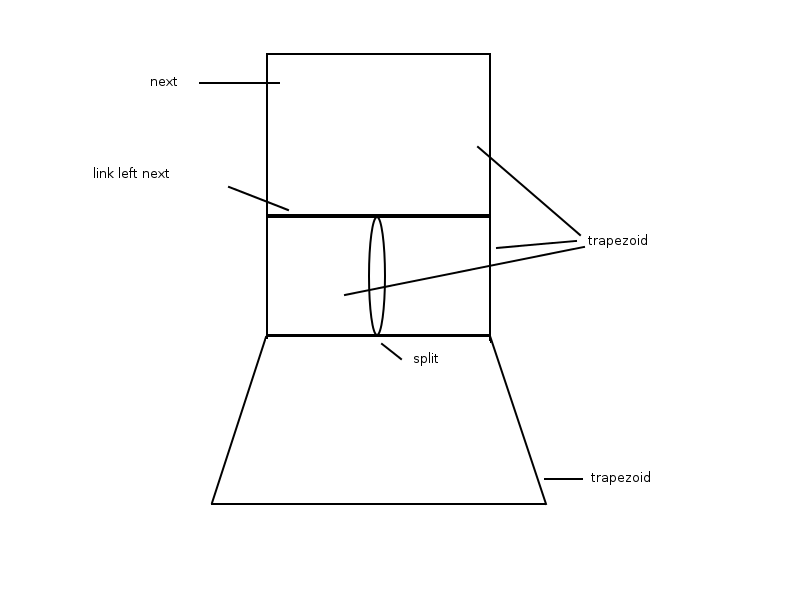
\includegraphics[scale=0.4]{../img/poncho.png}
  \caption{Le poncho généré par le code précédent}
  \label{poncho}
\end{figure}

La syntaxe a été définie et le parser utilisé par le traducteur a été implémenté.
Utiliser des trapèzes est selon nous intéressant, même lors de l'édition du tricot par l'utilisateur. En effet, chaque modification (ajout de points) correspondra à des séparations de trapèzes, ce qui est déjà géré par notre langage (via \texttt{split} et \texttt{link}). 


\subsection{Interface graphique}

Nous détaillons dans cette section les fonctionnalités implémentées jusqu'à présent au niveau de l'interface graphique.

\subsubsection{Squelette de l'interface / Aspect}

La première étape du développement de l'interface a été la mise en place de son squelette. Plus précisement, nous avons défini l'aspect
général de l'interface ainsi que les différents outils que nous souhaitons mettre à disposition. Ces outils sont représentés à l'aide de
boutons ou d'options encore inactives pour la plupart. On distingue notamment :
\begin{itemize}
  \item Les options relatives au logiciel TriComp (choisir un point, faire une tresse...) Ceux-ci peuvent être selectionnés grâce à des
boutons dont l'aspect n'est pas encore fixé, car leur implémentation se fera au fur et à mesure et en fonction de l'avancement global du
projet.
  \item Les options que l'on trouve dans tout logiciel (ouvrir, sauvegarder, quitter, ...). Ces options sont fonctionnelles (ou bientôt
fonctionnelles) car les formats de données pour la sauvegarde ont été définis. Nous travaillons directement sur le format de fichier
associé au langage descriptif. Ce type de fichier portera l'extension \texttt{.tricot}.
\end{itemize}
La figure \ref{fenetre} présente l'interface utilisateur du logiciel. Celle-ci se décompose en trois parties : 
\begin{enumerate}
   \item un panneau qui contiendra les différents outils de tricot mis à la disposition de l'utilisateur. Ces outils seront sous le forme de boutons ;
   \item une fenêtre d'affichage du tricot ;
   \item une fenêtre qui contiendra la liste des instructions générées par l'utilisateur.
\end{enumerate}

\begin{figure}[!h]
  \begin{center}
    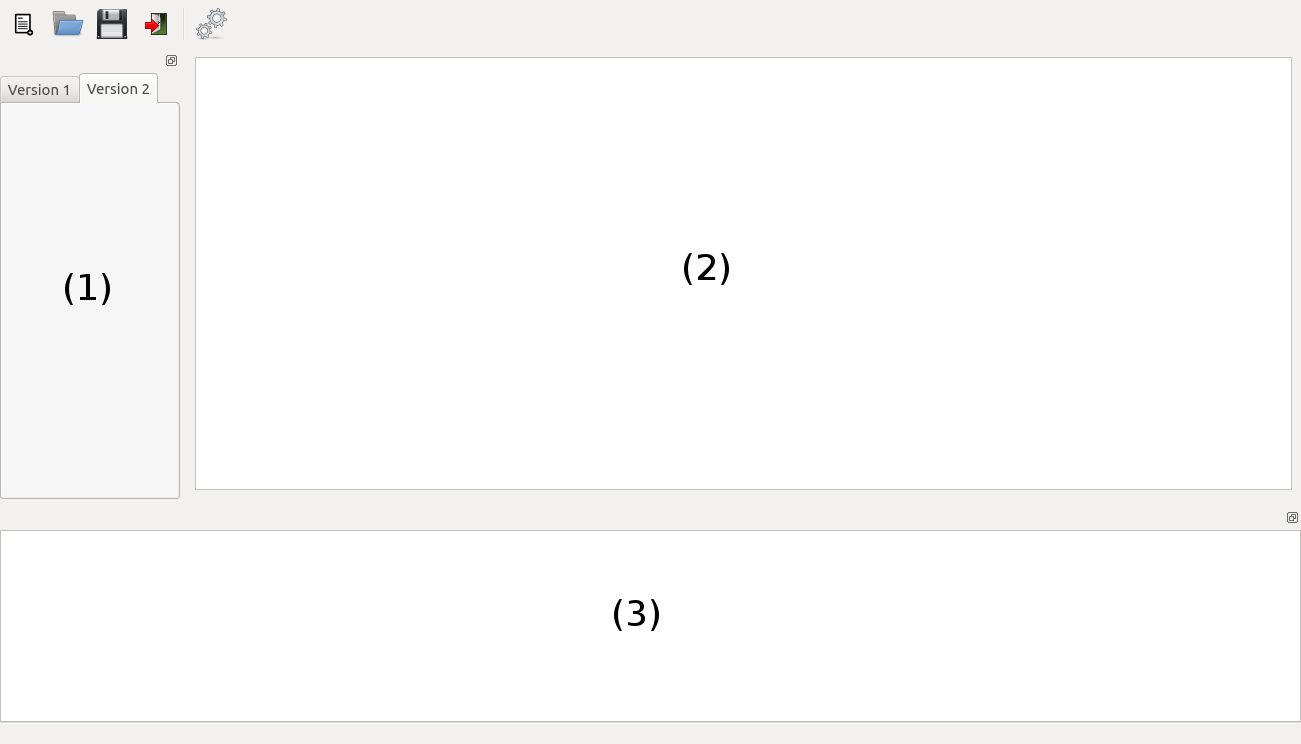
\includegraphics[scale=0.3]{fenetre.png}
  \end{center}
  \caption{L'aspect général de la fenêtre principale, avec les trois parties principales mises en évidence}
  \label{fenetre}
\end{figure}

\subsubsection{Affichage des tricots}

L'affichage des tricots en lui-même est en cours d'implémentation. Il est prévu de les afficher sous forme de patron, avec éventuellement
la possibilité d'afficher la progression d'un tricot en cours de réalisation.
Nous travaillons avec des classes de Qt qui permettent la gestion et l'affichage d'objets 2D (\texttt{QtGraphicsScene} et \texttt
{QtGraphicsItem} par exemple).

Nous avons également besoin d'un parser pour permettre l'utilisation du fichier \texttt{.tricot} par l'interface graphique. Celui-ci est 
sensiblement identique à celui implémenté en Ocaml et est en cours de finition (notamment son incorporation dans le projet Qt).

\subsection{Site Web}

Un site web a été déployé à l'adresse \url{http://tricomp.github.io}, il est hébergé sur Github (utilisé comme serveur Git du projet). Le
site est basé sur Jekyll, un CMS en Ruby spécialisé dans les blogs et qui a la particularité de ne pas utiliser de base de données, avec
l'avantage que Github gère Jekyll automatiquement. Le site est notament une vitrine pour le projet : il en contient une présentation
rapide, avec des liens vers le code source sur Github. A terme, le site sera aussi un support pour télécharger et installer le logiciel
TriComp.

De plus, le site contient pour l'instant un article sur ce qui existe déjà sur Internet autour du tricot (notamment certains projets
proches de TriComp qui ont été détaillés dans la proposition). D'autres articles devrait s'y rajouter, ainsi qu'une page pour aiguiller
rapidement l'internaute anglophone.

\section{Conclusion}

Malgré le travail fourni jusqu'à présent par toute l'équipe, tant du point de vue de la refléxion autour des différents langages que du code, la durée nécessaire à la mise en place d'une version entièrement fonctionelle du logiciel a été sous-estimée. Néanmoins, la durée nécessaire pour les nouvelles versions peut être revue à la baisse, car nos réflexions sur les différents aspects du projet ont permis d'avoir assez tôt une idée des difficultés qui nous attendent par la suite. 


\end{document}
